\apendice{Especificación de diseño}

\section{Introducción}
Tras haber definido los requisitos de la aplicación, es hora de definir el diseño de la aplicación. En este apartado se dará una descripción del diseño de los datos, el flujo de procedimientos y el diseño arquitectónico de la aplicación.

\section{Diseño arquitectónico}
Esta aplicación cuenta con una arquitectura Modelo-Vista-Controlador \cite{mvc}. Este es un patrón arquitectónico que divide la aplicación en tres componentes \ref{fig:mvc}:
\begin{itemize}
    \item \textbf{Modelo:} En este componente se encuentran los datos y toda la lógica relativa a su obtención.
    \item \textbf{Vista:} En la vista se encuentra la interfaz gráfica y todos aquellos componentes que interactúen directamente con el usuario.
    \item \textbf{Controlador:}Este componente es el intermediario entre el modelo y la vista, este es el que gestiona las peticiones que se reciben de la vista y decide que datos mostrar y como, es decir, es el que contiene la lógica de negocio.
\end{itemize}

\begin{figure}[H]
    \centering
    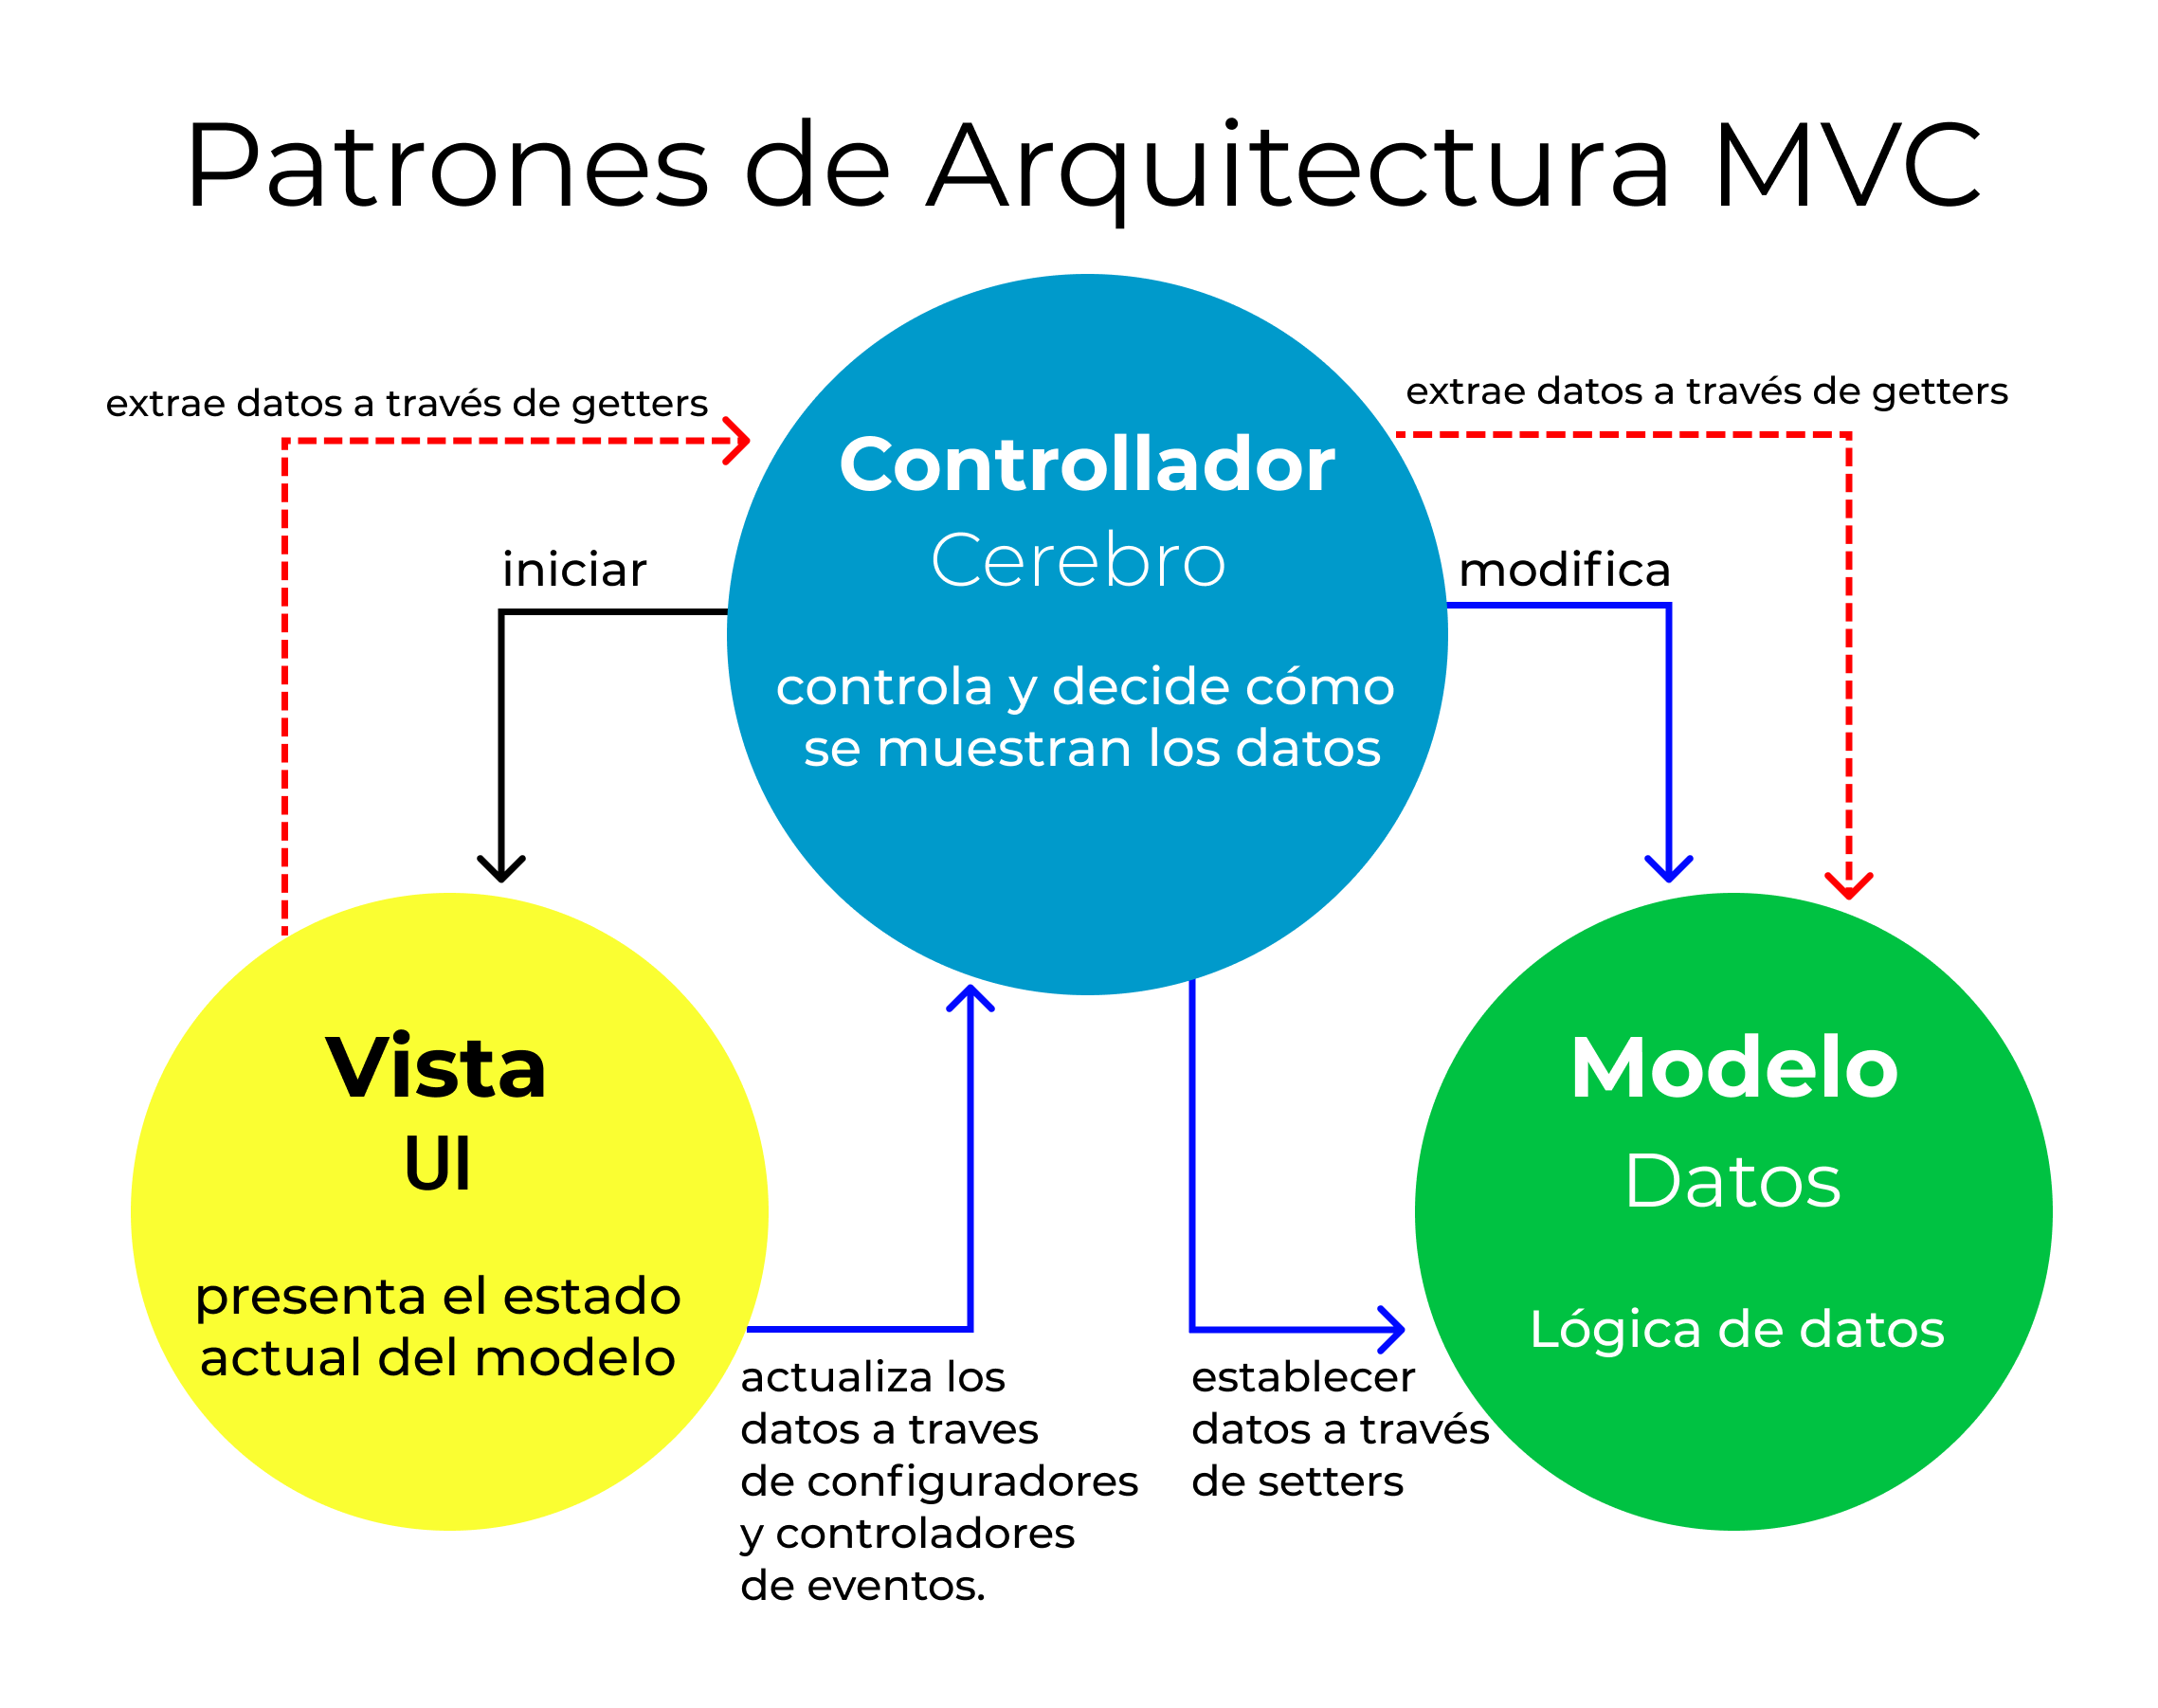
\includegraphics[width=1\linewidth]{img/MVC.png}
    \caption{Patrón Modelo-Vista-Controlador}
    \label{fig:mvc}
\end{figure}

En la aplicación se pueden encontrar estos componentes. En esta aplicación, el modelo para representar los datos obtenidos a través del web scraping o la Web API de Moodle. Este modelo se ve representado en la aplicación en la carpeta situada en src/main/java/es/ubu/lsi/model \ref{fig:modelo}:

\begin{figure}[H]
    \centering
    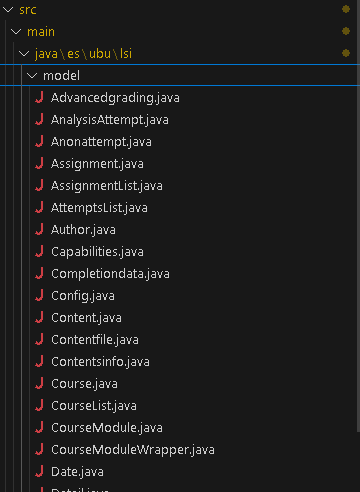
\includegraphics[width=0.6\linewidth]{img/modelo-elearningqa.png}
    \caption{Modelo de eLearningQA}
    \label{fig:modelo}
\end{figure}

La vista se ve representada en ficheros JSP en el paquete src/main/webapp. Aquí, se encuentra la interfaz de usuario y todos los métodos que utiliza. 

El controlador se encuentra en la aplicación\ref{fig:controlador} como un conjunto de clases que realizan las tareas propias a la lógica de negocio.

\begin{figure}[H]
    \centering
    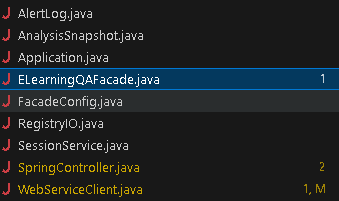
\includegraphics[width=0.5\linewidth]{img/controlador.png}
    \caption{Controlador en eLearningQA}
    \label{fig:controlador}
\end{figure}

Por otro lado, la aplicación cuenta con un patrón fachada, que centraliza los métodos que realizan las operaciones de la aplicación. Este patrón se implementa en la aplicación con una clase fachada llamada ElearningQAFacade que permite el aumento de funcionalidad sin que cambie mucho la fachada de la aplicación \ref{fig:diagrama-clases-elearningqa}.

\begin{figure}[H]
    \centering
    \includegraphics[width=1\linewidth]{patrón-fachada.png}
    \caption{Diagrama de clases de eLearningQA}
    \label{fig:diagrama-clases-elearningqa}
\end{figure}

\section{Diseño de datos}
Esta aplicación no dispone de persistencia de datos en base de datos. Hasta el momento, se guardan datos de los informes en archivos CSV que se utilizan para generar el gráfico de evolución de calidad. 

Sin embargo, sí que existe una gestión de los datos que se reciben desde la Web API de Moodle y del fichero estadístico de la web de Moodle. Estos datos se reciben en formato JSON y se realiza un cast a las entidades definidas en la capa de modelo de la aplicación en la aplicación. 

Las estructura de este Modelo gira en torno al curso, ya que los reportes se generan basándose en el curso. En la siguiente imagen \ref{fig:entidades} se puede ver la estructura de entidades de la que dispone la aplicación.

\begin{figure}[H]
    \centering
    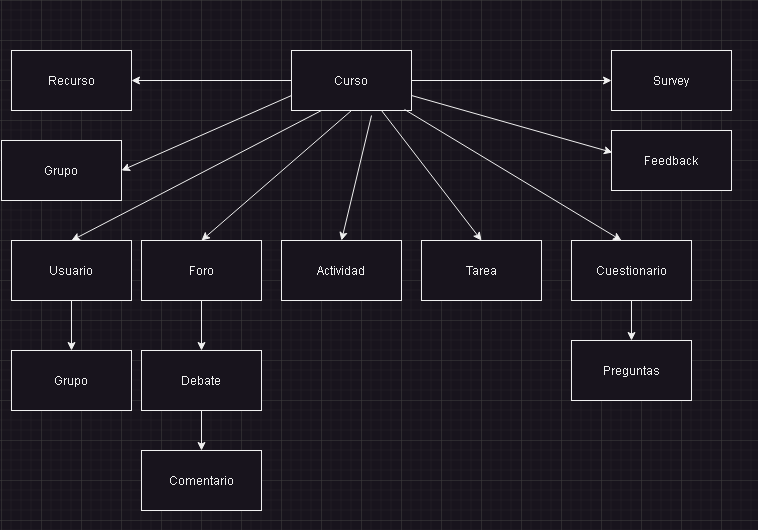
\includegraphics[width=1\linewidth]{img/entidades-modelo.png}
    \caption{Entidades del modelo de eLearningQA}
    \label{fig:entidades}
\end{figure}

\section{Diseño procedimental}
En este apartado se define el diseño procedimental que sigue la aplicación. La funcionalidad principal de la aplicación es la generación de informes de calidad. Para esta funcionalidad existe un conjunto de llamadas a distintos métodos en distintas clases \ref{fig:diseño-procedimental}.

\begin{figure}
    \centering
    \includegraphics[width=1\linewidth]{diseño-procedimental.png}
    \caption{Procedimiento de generación de un informe}
    \label{fig:diseño-procedimental}
\end{figure}

Como conclusión, es importante recalcar que este diseño debe ser revisado constantemente, como parte del proceso del mantenimiento. Ya que basándose en el crecimiento de necesidades, puede ser interesante un cambio estructural con el fin de mejorar le desarrollo de la aplicación en el largo plazo.



